\documentclass[10pt,ignorenonframetext,,aspectratio=149]{beamer}
\usefonttheme{serif} % use mainfont rather than sansfont for slide text
\setbeamertemplate{caption}[numbered]
\setbeamertemplate{caption label separator}{: }
\setbeamercolor{caption name}{fg=normal text.fg}
\usepackage{lmodern}
\usepackage{amssymb,amsmath}
\usepackage{ifxetex,ifluatex}
\usepackage{fixltx2e} % provides \textsubscript
\ifnum 0\ifxetex 1\fi\ifluatex 1\fi=0 % if pdftex
  \usepackage[T1]{fontenc}
  \usepackage[utf8]{inputenc}
\else % if luatex or xelatex
  \ifxetex
    \usepackage{mathspec}
  \else
    \usepackage{fontspec}
  \fi
  \defaultfontfeatures{Ligatures=TeX,Scale=MatchLowercase}
  \newcommand{\euro}{€}
    \setmainfont[]{Open Sans}
\fi
% use upquote if available, for straight quotes in verbatim environments
\IfFileExists{upquote.sty}{\usepackage{upquote}}{}
% use microtype if available
\IfFileExists{microtype.sty}{%
\usepackage{microtype}
\UseMicrotypeSet[protrusion]{basicmath} % disable protrusion for tt fonts
}{}
\usepackage{graphicx,grffile}
\makeatletter
\def\maxwidth{\ifdim\Gin@nat@width>\linewidth\linewidth\else\Gin@nat@width\fi}
\def\maxheight{\ifdim\Gin@nat@height>\textheight0.8\textheight\else\Gin@nat@height\fi}
\makeatother
% Scale images if necessary, so that they will not overflow the page
% margins by default, and it is still possible to overwrite the defaults
% using explicit options in \includegraphics[width, height, ...]{}
\setkeys{Gin}{width=\maxwidth,height=\maxheight,keepaspectratio}

% Comment these out if you don't want a slide with just the
% part/section/subsection/subsubsection title:
\AtBeginPart{
  \let\insertpartnumber\relax
  \let\partname\relax
  \frame{\partpage}
}
\AtBeginSection{
  \let\insertsectionnumber\relax
  \let\sectionname\relax
  \frame{\sectionpage}
}
\AtBeginSubsection{
  \let\insertsubsectionnumber\relax
  \let\subsectionname\relax
  \frame{\subsectionpage}
}

\setlength{\emergencystretch}{3em}  % prevent overfull lines
\providecommand{\tightlist}{%
  \setlength{\itemsep}{0pt}\setlength{\parskip}{0pt}}
\setcounter{secnumdepth}{0}

\title{Data Problems}
\author{Henrique Veras}
\date{}

%% Here's everything I added.
%%--------------------------

\usepackage{graphicx}
\usepackage{rotating}
%\setbeamertemplate{caption}[numbered]
\usepackage{hyperref}
\usepackage{caption}
\usepackage[normalem]{ulem}
%\mode<presentation>
\usepackage{wasysym}
%\usepackage{amsmath}


% Get rid of navigation symbols.
%-------------------------------
\setbeamertemplate{navigation symbols}{}

% Optional institute tags and titlegraphic.
% Do feel free to change the titlegraphic if you don't want it as a Markdown field.
%----------------------------------------------------------------------------------
\institute{PIMES/UFPE}

% \titlegraphic{\includegraphics[width=0.3\paperwidth]{\string~/Dropbox/teaching/clemson-academic.png}} % <-- if you want to know what this looks like without it as a Markdown field. 
% -----------------------------------------------------------------------------------------------------


% Some additional title page adjustments.
%----------------------------------------
\setbeamertemplate{title page}[empty]
%\date{}
\setbeamerfont{subtitle}{size=\small}

\setbeamercovered{transparent}

% Some optional colors. Change or add as you see fit.
%---------------------------------------------------
\definecolor{clemsonpurple}{HTML}{522D80}
 \definecolor{clemsonorange}{HTML}{F66733}
\definecolor{uiucblue}{HTML}{003C7D}
\definecolor{uiucorange}{HTML}{F47F24}


% Some optional color adjustments to Beamer. Change as you see fit.
%------------------------------------------------------------------
\setbeamercolor{frametitle}{fg=clemsonpurple,bg=white}
\setbeamercolor{title}{fg=clemsonpurple,bg=white}
\setbeamercolor{local structure}{fg=clemsonpurple}
\setbeamercolor{section in toc}{fg=clemsonpurple,bg=white}
% \setbeamercolor{subsection in toc}{fg=clemsonorange,bg=white}
\setbeamercolor{footline}{fg=clemsonpurple!50, bg=white}
\setbeamercolor{block title}{fg=clemsonorange,bg=white}


\let\Tiny=\tiny


% Sections and subsections should not get their own damn slide.
%--------------------------------------------------------------
\AtBeginPart{}
\AtBeginSection{}
\AtBeginSubsection{}
\AtBeginSubsubsection{}

% Suppress some of Markdown's weird default vertical spacing.
%------------------------------------------------------------
\setlength{\emergencystretch}{0em}  % prevent overfull lines
\setlength{\parskip}{0pt}


% Allow for those simple two-tone footlines I like. 
% Edit the colors as you see fit.
%--------------------------------------------------
\defbeamertemplate*{footline}{my footline}{%
    \ifnum\insertpagenumber=1
    \hbox{%
        \begin{beamercolorbox}[wd=\paperwidth,ht=.8ex,dp=1ex,center]{}%
      % empty environment to raise height
        \end{beamercolorbox}%
    }%
    \vskip0pt%
    \else%
        \Tiny{%
            \hfill%
		\vspace*{1pt}%
            \insertframenumber/\inserttotalframenumber \hspace*{0.1cm}%
            \newline%
            \color{clemsonpurple}{\rule{\paperwidth}{0.4mm}}\newline%
            \color{clemsonorange}{\rule{\paperwidth}{.4mm}}%
        }%
    \fi%
}

% Various cosmetic things, though I must confess I forget what exactly these do and why I included them.
%-------------------------------------------------------------------------------------------------------
\setbeamercolor{structure}{fg=blue}
\setbeamercolor{local structure}{parent=structure}
\setbeamercolor{item projected}{parent=item,use=item,fg=clemsonpurple,bg=white}
\setbeamercolor{enumerate item}{parent=item}

% Adjust some item elements. More cosmetic things.
%-------------------------------------------------
\setbeamertemplate{itemize item}{\color{clemsonpurple}$\bullet$}
\setbeamertemplate{itemize subitem}{\color{clemsonpurple}\scriptsize{$\bullet$}}
\setbeamertemplate{itemize/enumerate body end}{\vspace{.6\baselineskip}} % So I'm less inclined to use \medskip and \bigskip in Markdown.

% Automatically center images
% ---------------------------
% Note: this is for ![](image.png) images
% Use "fig.align = "center" for R chunks

\usepackage{etoolbox}

\AtBeginDocument{%
  \letcs\oig{@orig\string\includegraphics}%
  \renewcommand<>\includegraphics[2][]{%
    \only#3{%
      {\centering\oig[{#1}]{#2}\par}%
    }%
  }%
}

% I think I've moved to xelatex now. Here's some stuff for that.
% --------------------------------------------------------------
% I could customize/generalize this more but the truth is it works for my circumstances.

\ifxetex
\setbeamerfont{title}{family=\fontspec{Titillium Web}}
\setbeamerfont{frametitle}{family=\fontspec{Titillium Web}}
\usepackage[font=small,skip=0pt]{caption}
 \else
 \fi

% Okay, and begin the actual document...

\begin{document}
\frame{\titlepage}

\hypertarget{econometrics}{%
\section{Econometrics}\label{econometrics}}

\hypertarget{intro}{%
\subsection{Intro}\label{intro}}

\begin{frame}{Intro}
We now turn our attention to data problems.

\vfill

The analysis to this point has assumed that the data in hand,
\(\mathbf{X}\) and \(\mathbf{y}\), are well measured and correspond to
the assumptions of the model and to the variables described by the
underlying theory.

\vfill

The cases we will examine are:

\begin{enumerate}
\tightlist
\item
  Multicollinearity
\item
  Missing values
\item
  Influential observations and outliers
\end{enumerate}
\end{frame}

\hypertarget{multicollinearity}{%
\subsection{Multicollinearity}\label{multicollinearity}}

\begin{frame}{Multicollinearity}
\protect\hypertarget{multicollinearity-1}{}
One important thing to notice is that the Gauss-Markov theorem does not
guarantee that the LS estimator has a small variance in any absolute
sense.

\vfill

We can write the expression for the conditional variance of
\(\mathbf{b}_k\) in the following way.

\vfill

Define \(\mathbf{x}_k\) as the column of the matrix \(\mathbf{X}\)
associated with the data from variable \(k\).

\vfill

Moreover, define the matrix \(\mathbf{X}_{(k)}\) composed of the
remaining columns of \(\mathbf{X}\).

\vfill
\end{frame}

\begin{frame}{Multicollinearity}
\protect\hypertarget{multicollinearity-2}{}
Thus, we can write

\[Var[b_k|\mathbf{x}]=\frac{\sigma^2}{(1-R^2_k)\sum_{i=1}^n{(x_{ik}-\bar{x}_k)^2}}\]

\vfill

The factors that determine the precision of the \(k\)th LS coefficient
estimator are:

\begin{enumerate}
\item
  \(R_k^2\): greater \(R_k^2\) increases \(Var[b_k|\mathbf{x}]\) due to
  multicollinearity;
\item
  Variation in \(\mathbf{x}_k\): higher
  \(\sum_{i=1}^n{(x_{ik}-\bar{x}_k)^2}\) lowers \(Var[b_k|\mathbf{x}]\);
\item
  \(\sigma^2\): greater \(\sigma^2\) (poorer overall fit) increases
  \(Var[b_k|\mathbf{x}]\).
\end{enumerate}

\vfill
\end{frame}

\begin{frame}{When is multicollinearity a problem?}
\protect\hypertarget{when-is-multicollinearity-a-problem}{}
Some computer packages report a variance inflation factor (VIF):
\(1/(1-R_k^2)\).

\vfill

This is the increase in \(Var[b_k|\mathbf{x}]\) that can be attributed
to the correlation between the variables of the model.

\vfill

The general rule of thumb is that VIFs exceeding 4 warrant further
investigation, while VIFs exceeding 10 are signs of serious
multicollinearity requiring correction.

\vfill
\end{frame}

\begin{frame}{What to do when multicollinearity is a problem?}
\protect\hypertarget{what-to-do-when-multicollinearity-is-a-problem}{}
\begin{enumerate}
\tightlist
\item
  Get more data

  \begin{itemize}
  \tightlist
  \item
    But if more data is available, why would the analyst not use them to
    begin with?
  \end{itemize}
\item
  Drop variables causing the problem

  \begin{itemize}
  \tightlist
  \item
    This creates a dillema: bias vs.~precision.
  \end{itemize}
\end{enumerate}
\end{frame}

\begin{frame}{The multicolinearity dillema}
\protect\hypertarget{the-multicolinearity-dillema}{}
Consider the partitioned multiple regression

\[\mathbf{y}=\mathbf{X\beta}+z\gamma+\varepsilon\]

\vfill

If we regress \(\mathbf{y}\) on \(\mathbf{X}\) only, the estimator is
biased. Can you show this?

\vfill

Moreover, we can show that

\[Var[\mathbf{b|X}]\leq Var[\mathbf{b_{\mathbf{X.z}}|X}\]

\vfill

Thus, we have a tradeoff: omitting a variable from the model improves
precision but introduces bias.

\vfill
\end{frame}

\hypertarget{missing-values-and-data-imputation}{%
\subsection{Missing values and data
imputation}\label{missing-values-and-data-imputation}}

\begin{frame}{Missing values and data imputation}
\protect\hypertarget{missing-values-and-data-imputation-1}{}
When is it likely that some data is missing?

\begin{enumerate}
\tightlist
\item
  Surveys: some people might fail to answer questions.
\item
  Time series: some data measured at different frequencies;
\item
  Panel data: attrition
\end{enumerate}

\vfill
\end{frame}

\begin{frame}{Missing values and data imputation}
\protect\hypertarget{missing-values-and-data-imputation-2}{}
Cases to consider when data is missing:

\begin{enumerate}
\item
  Missing completely at random (MCAR): Affects efficiency but does not
  introduce any sort of bias on the estimated coefficients
\item
  Not missing at random (NCAR): Highly problematic, as it might
  introduce bias
\end{enumerate}

\vfill
\end{frame}

\begin{frame}{Data imputation methods}
\protect\hypertarget{data-imputation-methods}{}
To improve efficiency, we can input some information on the missing
observations:

\vfill

\begin{enumerate}
\tightlist
\item
  Zero-order method: Replacing missing \(x\) with \(\bar{x}\) is
  equivalent to dropping the incomplete data.
\item
  Use the regression model to input the data.
\end{enumerate}

\vfill

It is important to notice, however, that all methods introduce some sort
of \emph{measurement error}, which causes bias (more on measurement
error and what to do later on the course!)

\vfill
\end{frame}

\hypertarget{outliers-and-influential-observations}{%
\subsection{Outliers and Influential
Observations}\label{outliers-and-influential-observations}}

\begin{frame}{Influential Observations}
\protect\hypertarget{influential-observations}{}
Given that the LS method is based on the \emph{squared} deviations, the
estimation is likely to be influenced by \textbf{extreme} observations.

\vfill

An \emph{influential} observation is one that is likely to have a
substantial impact on the LS coefficients.

\vfill

We can define an influence measure for observation \(\mathbf{x}_i\) as

\[h_i = \frac{1}{n}+\frac{(x_i-\bar{x}_{(i)})^2}{\sum_{j\neq i}^n{(x_j-\bar{x}_{(i)})^2}}\]

\vfill

We can say an observation is influential if \(h_i>2/n\).

\vfill

Notice that the analysis is conditional on \(x_i\) only.

\vfill
\end{frame}

\begin{frame}{Influential Observations}
\protect\hypertarget{influential-observations-1}{}
What happens to the linear regression coefficient vector in a multiple
regression when one observation is added to the sample?

\vfill

We can show that the change in the linear coefficient is

\[\mathbf{b}-\mathbf{b_{(i)}}=\Delta \mathbf{b}= \frac{1}{1+\mathbf{x}_i'(\mathbf{X}_{(i)}'\mathbf{X}_{(i)})^{-1}\mathbf{x}_i}(\mathbf{X}_{(i)}'\mathbf{X}_{(i)})^{-1}\mathbf{x}_i(\mathbf{y}_i-\mathbf{x}_i'\mathbf{b_{(i)}})\]

\vfill

\(\mathbf{b}\) is computed with observation \(i\) and
\(\mathbf{b_{(i)}}\) is computed without it.

\vfill

An influential measure that is used is

\[h_{ii}=mathbf{x}_i'(\mathbf{X}_{(i)}'\mathbf{X}_{(i)})^{-1}\mathbf{x}_i\]

\vfill

The selection criterion would be \(h_{ii}>2(K-1)/n\).

\vfill
\end{frame}

\begin{frame}{Outliers}
\protect\hypertarget{outliers}{}
\emph{Outliers} are observations that seem to come from outside the DGP/

\vfill

Some reasons for outliers on the data:

\begin{enumerate}
\tightlist
\item
  Data error
\item
  Unusual residuals
\item
  Observation coming from a different population
\end{enumerate}

To test for this latter case, we can construct \emph{studentized
residuals} by computing the regression coefficients and the residual
variance without observation \(i\) for each observation in the sample
and then standardizing the modified residuals.

\vfill
\end{frame}

\begin{frame}{Outliers}
\protect\hypertarget{outliers-1}{}
The \(i\)th studentized residual is

\[e(i)=\frac{e_i / \sqrt{1-h_{ii}}}{\sqrt{\frac{\mathbf{e'e}-e_i^2(1-h_{ii})}{n-1-K}}}\]

\vfill

Observations with \(e(i)>2\) would be considered outliers.

\vfill

Using this procedure might be problematic as it should raise skepticism
about the model specification in case a substantial proportion of the
observations are considered outliers.

\vfill
\end{frame}

\begin{frame}{Outliers and Influential Points Graphically}
\protect\hypertarget{outliers-and-influential-points-graphically}{}
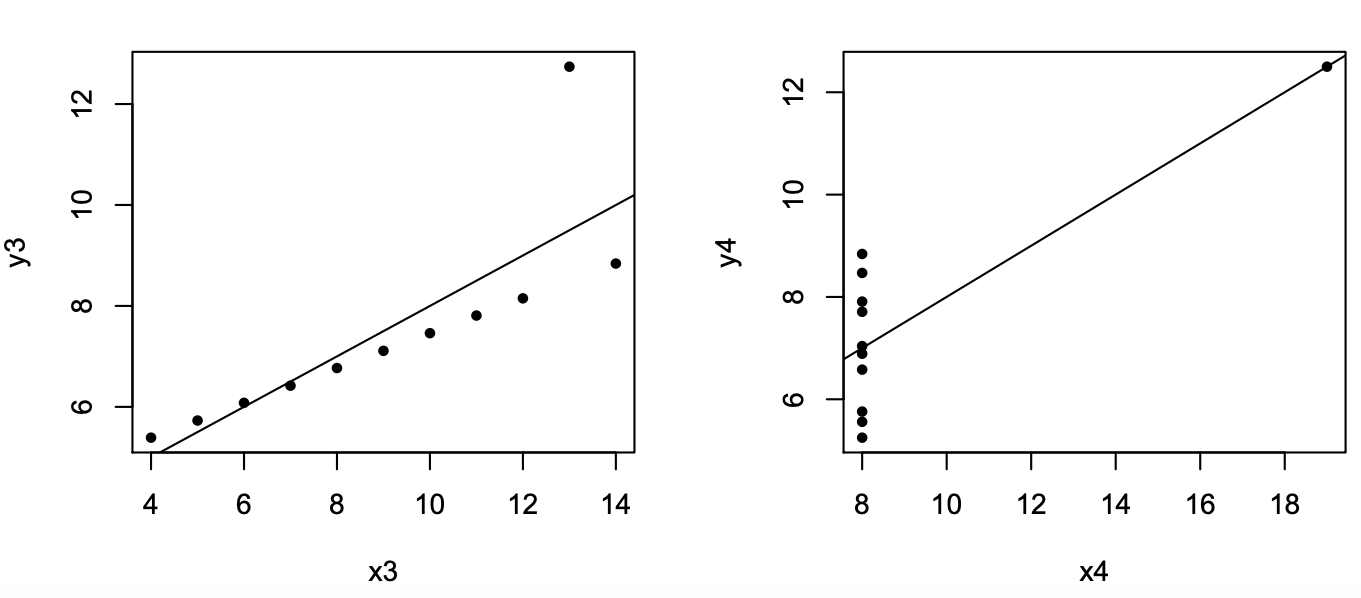
\includegraphics{/Users/henriquefonseca/Desktop/temp/Rmarkdown-practice/henriqueveras.github.io/files/Econometrics/Lecture Notes/4/outlier-leverage.png}
\end{frame}


\section[]{}
\frame{\small \frametitle{Table of Contents}
\tableofcontents}
\end{document}
